% Extension paper: structure learning of agency with tensor networks.
% Builds on "Characterizing Agency in AI Systems" (Wilson et al.), promoting the
% learned-model pipeline from a companion section to the central contribution.
\documentclass[runningheads]{llncs}
\usepackage[T1]{fontenc}
\usepackage{graphicx}
\usepackage{amsmath}
\usepackage{amssymb}
\usepackage{booktabs}
\PassOptionsToPackage{hyphens}{url}
\usepackage{hyperref}
\renewcommand\UrlFont{\color{blue}\rmfamily}
\urlstyle{rm}

\begin{document}

\title{Structure Learning of Agency: Recovering Interpretable Generative Models
from Behaviour with Tensor Networks}
\titlerunning{Structure Learning of Agency}

\author{Philip Wilson\inst{1} \and
Mahault Albarracin\inst{2,3} \and
Nicol\'{a}s Hinrichs\inst{4} \and
Jasmine Moore\inst{1} \and
Daniel Polani\inst{5} \and
Karl J. Friston\inst{6} \and
Axel Constant\inst{7}}
\authorrunning{P. Wilson et al.}
\institute{Independent Researcher \and
LANCI, Universit\'{e} du Qu\'{e}bec \`{a} Montr\'{e}al, Canada \and
Centre of Excellence for AI and Robotics, Sheffield Hallam University, UK \and
Max Planck Institute for Human Cognitive and Brain Sciences, Leipzig, Germany \and
University of Hertfordshire, Hatfield, UK \and
Wellcome Centre for Human Neuroimaging, UCL, London, UK \and
University of Sussex, Brighton, UK}

\maketitle

\begin{abstract}
This paper is a direct follow-up to our prior work on characterising agency in AI
systems, which proposed a three-criterion definition of agency (intentionality,
rationality, explainability), cast empowerment as a probe of control capacity, and---on
\emph{hand-specified} generative models---carried out only the second half of
computational phenotyping: reading agency-relevant quantities off a model. Here we
carry out the first half. A matrix product state (an interpretable tensor network) is
trained unsupervised on action--observation rollouts of a T-maze partially observable
Markov decision process, so its generative model $p(o,a)$ is learned from data rather
than stipulated; we then recover the model's structure in five senses that a bare
density estimate does not provide, and show that once the model is learned the readout
returns the entire interpretable model behind the number. From the learned network
we (i) extract normalised hidden states by a gauge-invariant, predictive-equivalence
criterion---closing a gap left open by earlier tensor-network work, whose bond
indices were ``not normalised and therefore not usable''; (ii) reconstruct the
labelled likelihood $A=p(o\mid s)$ and transition $B=p(s'\mid s,a)$ and match them to
the ground-truth environment (emission total-variation $0.000$, transition branching
exact); (iii) recover the conditional-independence structure by exact mutual
information; (iv) discover that the observation factorises, with context a
near-independent modality; and (v) select the number of hidden states by a
model-selection criterion rather than a truncation threshold, which we cast as active
inference model expansion and Bayesian model reduction. On the learned model we then
phenotype control capacity: empowerment reproduces the analytic zero-, intermediate-,
and maximal-control regimes to three decimals, and epistemic action increases
empowerment without it being an explicit objective. The pipeline is
architecture-agnostic---the tensor network is not itself an active-inference
agent---so the criteria and probe apply to any system whose sensorimotor stream can
be modelled.
\keywords{Active inference \and Agency \and Computational phenotyping \and
Empowerment \and Tensor networks \and Structure learning \and World models}
\end{abstract}

\section{Introduction}\label{sec:intro}

Agency in artificial systems is increasingly asserted and rarely measured. In a first
paper~\cite{wilsonAgency2025} (hereafter Paper~I) we argued that a minimal, operational
notion of agency rests on three criteria---\emph{intentionality} (action grounded in
beliefs and desires), \emph{rationality} (normatively coherent action entailed by a
world model), and \emph{explainability} (action causally traceable to internal
states)---and that active inference~\cite{parr2022} realises all three jointly in a
partially observable Markov decision process (POMDP), whose likelihood and transition
tensors constitute an inspectable world model. On that model, \emph{empowerment}---the
channel capacity between actions and future observations~\cite{klyubin2005,salge2014}
---serves as an operational probe of the control capacity that intentional action
presupposes. This paper is the direct follow-up: it takes the definition, the probe,
and the T-maze of Paper~I as given, and supplies the piece Paper~I explicitly deferred.

That programme borrows its method from computational psychiatry's
\emph{phenotyping}~\cite{montague2012,schwartenbeck2016}: (i) fit a generative model
to behavioural data, and (ii) explain variation from the inferred parameters. Paper~I
performed only the second half, on models specified by hand, and sketched the first as
a companion pipeline. Here we build that pipeline, and show that once the model is
learned from behaviour the second half returns not just a number but the entire
interpretable model behind it.

Concretely, we train a \emph{matrix product state} (MPS), a one-dimensional tensor
network, as an unsupervised generative model of T-maze rollouts, following
Wauthier~et~al.~\cite{wauthier2022}. Tensor networks are attractive here because they
admit exact marginalisation: the conditionals the empowerment probe needs, and the
mutual informations a dependency analysis needs, are available in closed form from
reduced density matrices. But a trained density model is not yet a \emph{structured}
one. Wauthier~et~al.\ observed that although the bonds between tensors ``can be
regarded as internal states, they are not normalised and therefore not usable,'' and
consequently bypassed hidden-state recovery entirely. Our central technical
contribution is to supply exactly that missing piece and to build a full structural
readout on top of it.

\paragraph{Contributions.} From MPS models trained on the minimal four-observation
T-maze and the full \texttt{pymdp} T-maze (24 composite observations), we recover, and
validate against analytic ground truth:
\begin{enumerate}
\item \textbf{Hidden states} by gauge-invariant fidelity clustering, corrected to a
\emph{predictive-equivalence} criterion that is robust to gauge coherences the model
writes into the bond (Sec.~\ref{sec:states});
\item \textbf{A labelled generative model}: emission $A=p(o\mid s)$ and transition
$B=p(s'\mid s,a)$, matched to the environment up to a state permutation
(Sec.~\ref{sec:ab});
\item the \textbf{conditional-independence graph} over observables, by exact mutual
information (Sec.~\ref{sec:graph});
\item the \textbf{observation factorisation}, from subsystem mutual information of the
single-site reduced density matrix (Sec.~\ref{sec:factor});
\item the \textbf{number of hidden states} by model selection, framed as active
inference model expansion and Bayesian model reduction (Sec.~\ref{sec:modelsel}); and
\item \textbf{symbolic states}: a gauge that makes the bond index itself a labelled
hidden state (Sec.~\ref{sec:gauge}).
\end{enumerate}
On the learned model we then phenotype control capacity (Sec.~\ref{sec:empower}). All
code accompanies the paper.

\section{Background}\label{sec:background}

We recap only what the pipeline needs; the three agency criteria, the empowerment
probe, and the design of the T-maze are developed in full in Paper~I~\cite{wilsonAgency2025},
and the tensor-network machinery is new to this paper.

\subsection{The task and the analytic model}
The minimal T-maze is a two-step POMDP with three actions (Left, Right, Cue) and four
observations (Cheese, Shock, Left, Right); cheese and shock are placed left/right with
probability $1/2$ and the cue reveals their location, while entering an arm is an
absorbing trap (Fig.~\ref{fig:tmaze})~\cite{wilsonAgency2025}. The full
\texttt{pymdp}~\cite{heins2022pymdp} T-maze factors the observation into Position
($4$), Reward ($3$), and Context ($2$), yielding $24$ composite observations over a
three-step episode beginning with a null action. Both admit an exact generative model
$q(o,a)$, which we use only as ground truth for validation---the learner never sees it.

\begin{figure}[t]
\centering
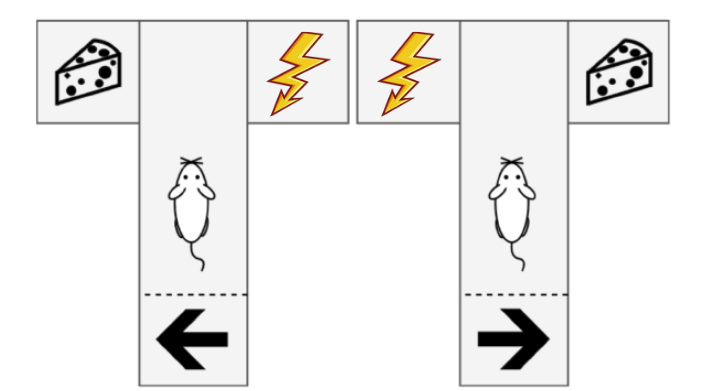
\includegraphics[width=0.42\textwidth]{figs/tmaze.png}
\caption{The T-maze. The arrow marks the observation revealing where the cheese is;
entering an arm is an absorbing trap, so the epistemically optimal first move is the
cue.}
\label{fig:tmaze}
\end{figure}

\subsection{MPS as a generative model}
An MPS represents the amplitude of a length-$L$ sequence as a chain of contracted
tensors, one per time step, each carrying a physical index (here the pair
[action,\,observation]) and two bond indices. Trained by the Born rule
$p(x)=|\psi(x)|^2/Z$~\cite{han2018}, it is a \emph{Born machine}, and admits exact
contraction of any marginal or conditional. Non-negative MPS are exactly hidden Markov
models, with the bond index a classical hidden state~\cite{glasser2019}; a generic
complex Born machine is strictly more expressive and has no such exact form, so hidden
states must be recovered rather than read off (Sec.~\ref{sec:states}). We train each
model with a DMRG-style cumulant gradient sweep and a learning-rate schedule that
shrinks the step when the loss stalls~\cite{han2018}; the minimal model reaches
$\|p-q\|_1=0.13$ and the full model $\|p-q\|_1=0.005$.

\subsection{Empowerment}
Empowerment at a state is the channel capacity between the next action and the next
observation, $\max_{p(a)} I(A;O')$, computed by the Blahut--Arimoto
algorithm~\cite{salge2014}. Under the true environment conditional it is
\emph{objective} empowerment; under the agent's (here, the learned model's) conditional
it is \emph{subjective} empowerment, and the two coincide as the fit improves. We
report subjective potential empowerment over the full observation and over the reward
modality alone (the preference-relevant variant).

\section{Recovering hidden states}\label{sec:states}

The bond of a trained MPS is defined only up to a gauge transformation
$A^{(n)}\!\to A^{(n)}G,\ A^{(n+1)}\!\to G^{-1}A^{(n+1)}$, so the bare bond index has no
intrinsic labelling. We first fix states in a gauge-invariant way: each
action--observation history $h$ induces a bond vector $|b_h\rangle$, and histories are
clustered by pairwise fidelity $|\langle b_i|b_j\rangle|^2$
(Fig.~\ref{fig:states}, left/centre).

On the minimal maze this yields exactly four states (cheese-trap, shock-trap, and one
per cue context), merging the two arms of entry because position is unobservable
there. On the full maze, however, raw fidelity clustering \emph{over-separates}: the
model writes the uninformative context bit of the mid-step observation into the bond
as a coherence that does not affect the future, splitting otherwise-identical states.
The robust criterion is \emph{predictive equivalence}---the predictive-state /
observable-operator definition of state~\cite{hsu2012,srinivasan2021}: two histories
are the same state iff they induce the same future conditional
$p(o'\mid a',h)$. Clustering the action-conditioned predictive signatures, and cutting
the dendrogram at its largest gap (Fig.~\ref{fig:states}, right), collapses the gauge
duplicates and returns the correct seven states (unresolved start, four arm--outcome
traps, two cue contexts). The learned state space thus tracks distinguishability, not
surface history---arm-of-entry histories merge when position is hidden and separate
when it is observed.

\begin{figure}[t]
\centering
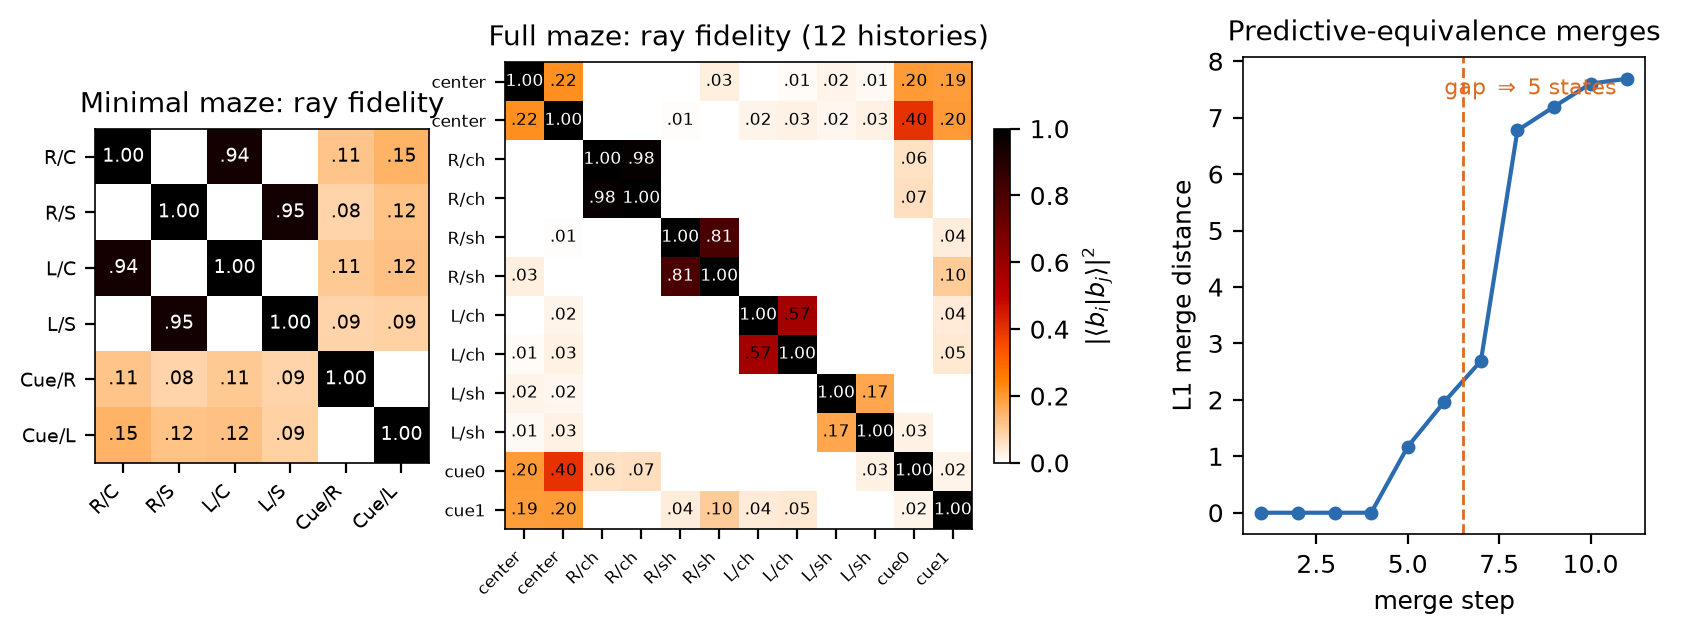
\includegraphics[width=\textwidth]{figs/fig_states.png}
\caption{State recovery. Pairwise bond-ray fidelity for the minimal maze (left, four
blocks) and full maze (centre); raw fidelity over-separates on the full maze because
the uninformative context bit is written into the bond. Right: predictive-equivalence
merge distances---the near-zero merges collapse the gauge duplicates and the gap fixes
the count at seven.}
\label{fig:states}
\end{figure}

\section{A labelled generative model: emission and transition}\label{sec:ab}

Given the states, we reconstruct the factorised model. Because probabilities are
Born-squared, we push amplitudes to probabilities \emph{before} forming any stochastic
object: attempting to read a stochastic matrix off the complex tensor, or to
gauge-transform the model into a non-negative form, is either ill-defined or NP-hard
for a genuine Born machine~\cite{glasser2019}. The \textbf{emission}
$A=p(o\mid s)$ is estimated by conditioning the exact joint on each state's histories
and marginalising the action; the \textbf{transition}
$B=p(s'\mid s,a)$ by re-contracting the bond after appending $(a,o)$, classifying the
resulting state by predictive equivalence, and accumulating Born weight. States are
matched to the environment by the Hungarian algorithm, the only residual gauge freedom
being a discrete permutation.

The reconstruction is essentially exact (Fig.~\ref{fig:ab}, Table~\ref{tab:results}).
On the minimal maze the emission matches ground truth to total-variation $0.000$ for
all four states. On the full maze, all seven emissions match to mean total-variation
$0.000$: the four traps are deterministic, and the two cue states carry the correct
\emph{opposite} action-conditioned reward patterns (under Right, context~0 yields
cheese and context~1 yields shock). The recovered transition reproduces the branching
structure of the environment exactly: from the start, Right and Left each split
$0.50/0.50$ over their two arm--outcome states, Cue splits $0.50/0.50$ over the two
context states, and staying at the centre is deterministic. This is the object
Wauthier~et~al.\ could not extract: a normalised, labelled, ground-truth-comparable
$A$ and $B$ read from a network trained on behaviour alone.

\begin{figure}[t]
\centering
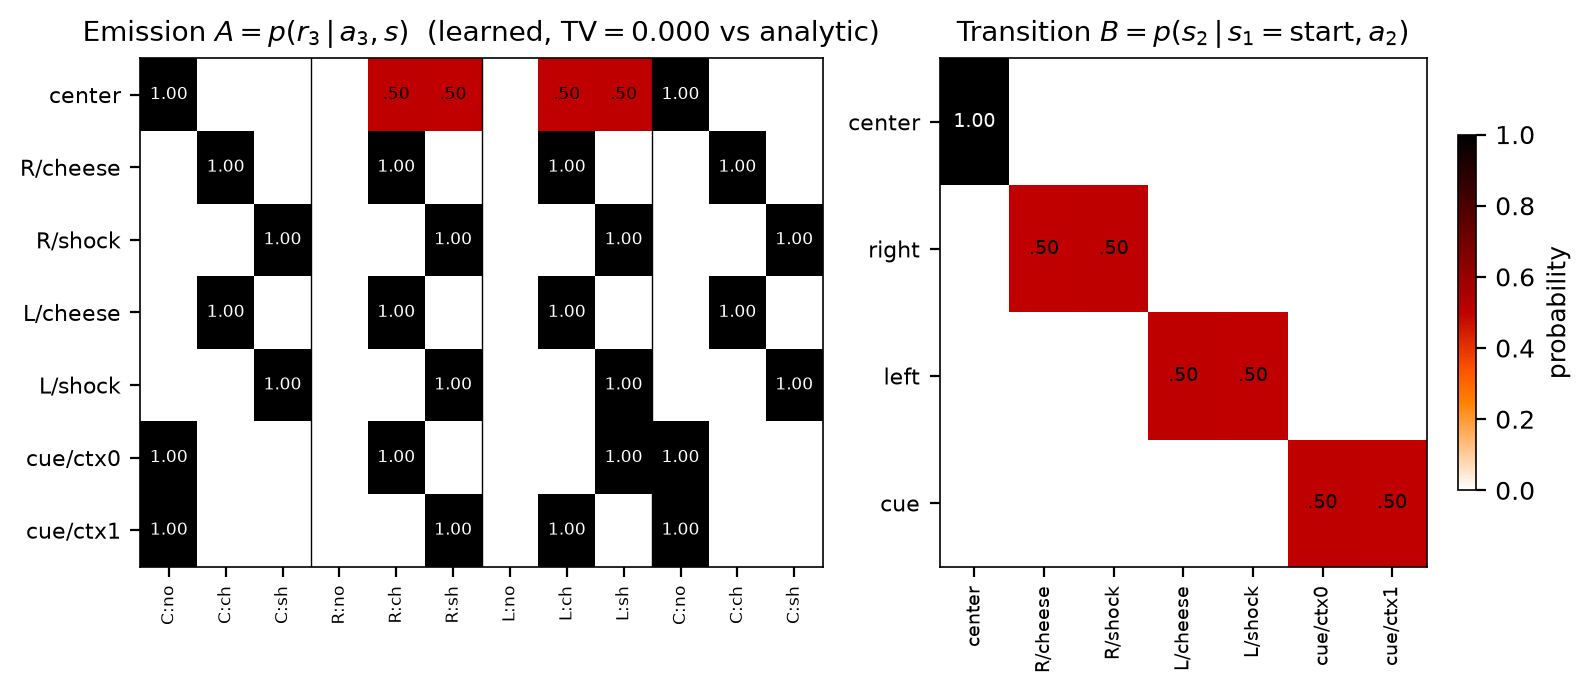
\includegraphics[width=\textwidth]{figs/fig_ab.png}
\caption{Recovered generative model (full maze). Left: emission
$A=p(r_3\mid a_3,s)$ over seven states and four actions $\times$ three rewards; each
state's pattern matches analytic ground truth (mean TV $0.000$). Right: transition
$B=p(s_2\mid s_1{=}\text{start},a_2)$, recovering the exact $0.50/0.50$ arm and cue
branching.}
\label{fig:ab}
\end{figure}

\section{The dependency graph}\label{sec:graph}

Because the learned joint is available in closed form, its dependency structure
follows from exact mutual information. We form the pairwise MI matrix over the observed
variables and take its maximum-weight spanning tree (Chow--Liu~\cite{chowliu1968}), the
tensor-network analogue of reading correlation structure off a quantum
state~\cite{rissler2006} (Fig.~\ref{fig:graph}). The recovered tree is the correct
temporal chain: the action at each step is strongly coupled to its observation and the
observation to the next. Conditional mutual information supplies exact
independence certificates: $I(a_1;o_3\mid o_2)=0$ (the first action affects the last
observation only through the intervening one) and, in the minimal maze,
$I(a_1;o_3\mid o_2)=0$ with $I(o_2;o_3\mid a_2)=1.31$ bits (dependence where the model
should be dependent). We validate against the \emph{observable-projected} ground-truth
graph, since marginalising the latent state induces real dependencies among
observables that a naive comparison to the full dynamic Bayes net would misread as
error.

\begin{figure}[t]
\centering
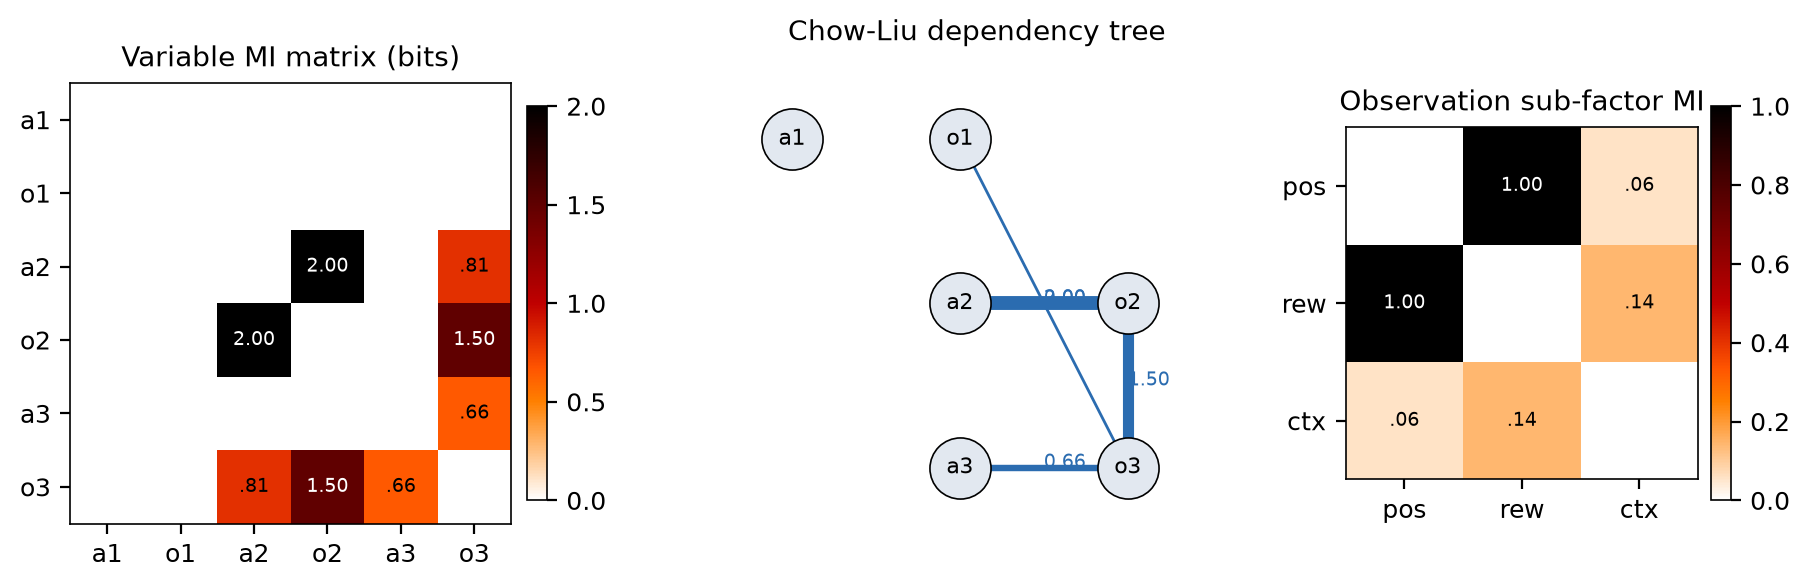
\includegraphics[width=\textwidth]{figs/fig_graph.png}
\caption{Dependency and factorisation (full maze). Left: pairwise mutual-information
matrix over the six observed variables. Centre: the Chow--Liu tree recovers the
temporal action--observation chain. Right: subsystem mutual information of the
single-site reduced density matrix---the model discovers context as a near-independent
factor ($I(\text{pos:ctx}),I(\text{rew:ctx})\approx0.05$) while position and reward are
coupled ($1.0$ bit), the causally correct structure.}
\label{fig:graph}
\end{figure}

\section{Discovering the observation factorisation}\label{sec:factor}

The full-maze model is fed a \emph{flat} 24-dimensional observation; the
Position$\times$Reward$\times$Context factorisation is assumed only in analysis. We
test whether the learned tensors respect it, from the single-site reduced density
matrix $\rho=\mathrm{Tr}_{\text{rest}}|\psi\rangle\langle\psi|$. Subsystem quantum
mutual information $I(A{:}B)=S(\rho_A)+S(\rho_B)-S(\rho_{AB})$ vanishes iff the factors
are independent~\cite{convy2022}. The model discovers context as a
\emph{near-independent} modality ($I(\text{pos:ctx}),I(\text{rew:ctx})\approx0.05$
bits) while position and reward remain coupled ($1.0$ bit)---which is causally correct,
since position gates whether a reward is possible (Fig.~\ref{fig:graph}, right). A
search over groupings of the 24 indices confirms it: the trace-distance residual
$\tfrac12\|\rho-\bigotimes_k\rho_k\|_1$ is far lower for
$(\text{position},\text{reward})\times\text{context}$ ($0.21$) than for full separation
($0.54$). The model organises the observation along the environment's causal axes
without being told they exist.

\section{Selecting the number of states}\label{sec:modelsel}

That the recovered dimensionality is a \emph{model-selection} result, not an artefact
of an SVD threshold, is shown by sweeping the capped bond dimension $\chi$ and training
each model to convergence (Fig.~\ref{fig:modelsel}). On the minimal maze the fit
improves sharply until $\chi=4$ (fit L1 $0.17\!\to\!0.03$) and then goes flat: extra
bond dimension is unused ``spare capacity.'' We read this through active inference
structure learning~\cite{friston2019bmr,smith2020}: a large-$\chi$ model has spare
capacity; training commits capacity to states that raise model evidence
(accuracy gain exceeding complexity cost) and leaves the rest unused, so the selected
count is the fixed point of a free-energy trade-off over model structure---model
expansion followed by Bayesian model reduction. A description-length penalty is
one state more conservative here, because the fourth state adds interpretable
low-probability structure that the fit needs but the likelihood barely rewards; the
$L_1$ knee is the decisive signal.

\begin{figure}[t]
\centering
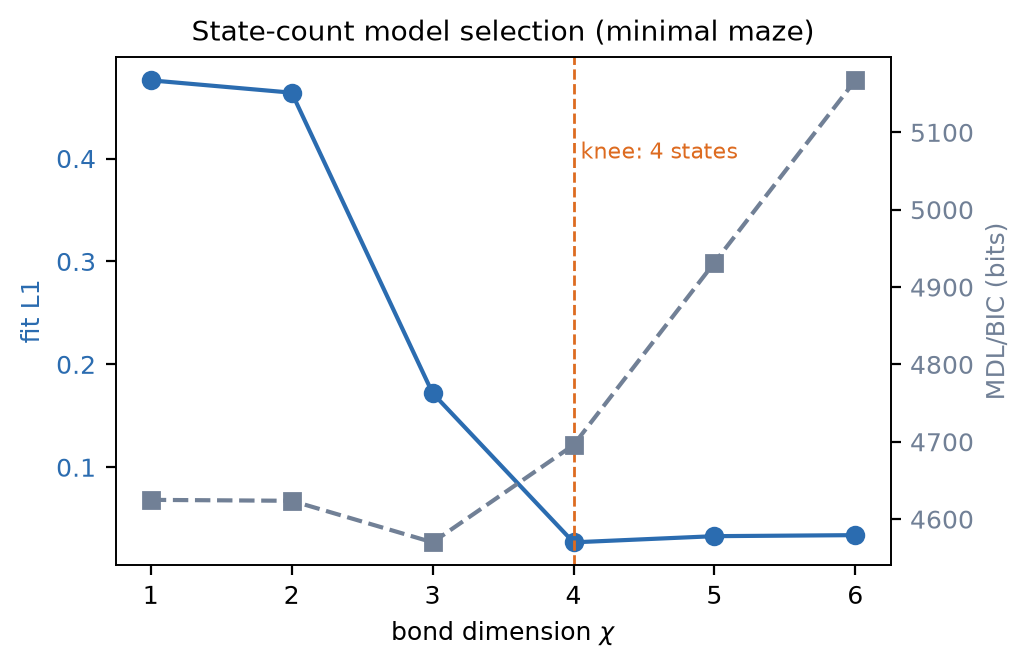
\includegraphics[width=0.62\textwidth]{figs/fig_modelsel.png}
\caption{State-count selection (minimal maze). Fit L1 (blue) drops $\sim$6$\times$ from
$\chi=3$ to $\chi=4$ and then plateaus; bond dimension beyond four is spare capacity.
The description-length score (grey) is one state more conservative.}
\label{fig:modelsel}
\end{figure}

\section{Symbolic states by gauge fixing}\label{sec:gauge}

Finally we remove the post-hoc character of state extraction by choosing the residual
gauge that rotates the bond into the cluster basis. From the $k$ cluster
representatives we build an orthonormal frame (the eigenbasis of the history-aggregated
bond density is more robust than a raw QR) and complete it to a unitary $U$; applying
$U$ as the gauge preserves the represented distribution exactly (here to
$4\times10^{-14}$) while the bond index becomes a labelled state that the model
\emph{emits}, $p_i(h)=|\langle q_i|U^\dagger|b_h\rangle|^2$
(Fig.~\ref{fig:empower}, right)~\cite{orus2014,aizpurua2024}. On the minimal maze the
emitted distributions agree with the fidelity clustering (adjusted Rand index $1.0$),
near one-hot for the trap states and softer for the cue states---the expected signature
of a genuinely complex Born machine, for which an exact classical-state gauge does not
exist~\cite{glasser2019}, quantified rather than hidden.

\section{Phenotyping control capacity on the learned model}\label{sec:empower}

With the model recovered, we phenotype it. Subjective potential empowerment computed
from the converged full-maze network reproduces the analytic regimes essentially
exactly (Fig.~\ref{fig:empower}, left; Table~\ref{tab:results}): $2.00$ bits at the
start, $0.00$ in the trap, and $2.00$ bits (full) / $1.585$ bits (reward) post-cue,
against analytic $2.00$/$1.585$. The reward-modality restriction recovers the three
control regimes of the minimal maze ($1.00$/$0.00/1.585$ bits), so restricting the
probe to preferred modalities surfaces the agency-relevant structure that the full
observation space obscures. The subjective--objective gap is now empirical and small:
a bond-truncated checkpoint attenuates post-cue empowerment ($0.65$ bits reward-only),
and it approaches the objective value as the fit improves. Epistemic action increases
empowerment---the cue raises it from the intermediate to the maximal regime---without
empowerment being any part of the training objective.

\begin{figure}[t]
\centering
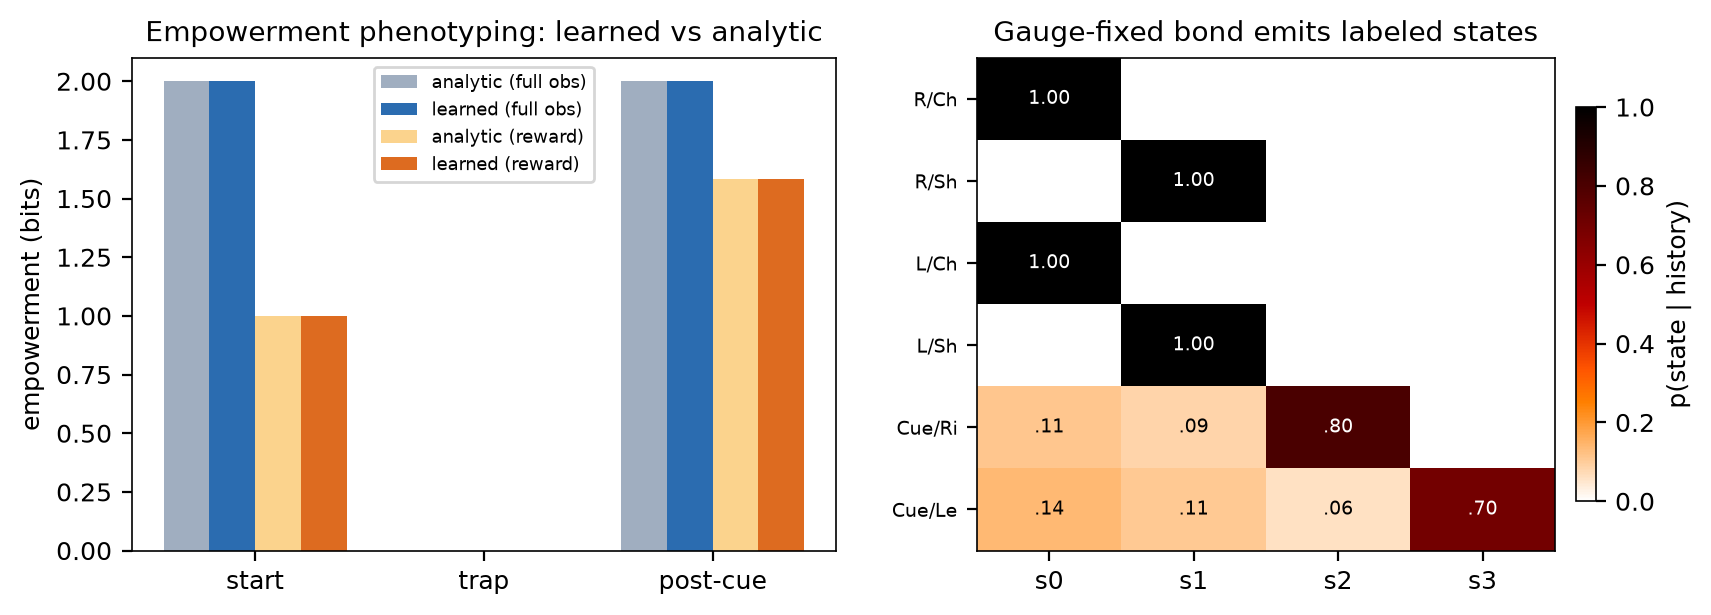
\includegraphics[width=\textwidth]{figs/fig_empower.png}
\caption{Left: empowerment phenotyping on the learned full-maze model matches analytic
across the zero-, intermediate-, and maximal-control regimes, full-observation and
reward-only. Right: the gauge-fixed bond emits labelled states (minimal maze); trap
histories are near one-hot, cue histories softer.}
\label{fig:empower}
\end{figure}

\begin{table}[t]
\centering
\caption{Structure recovery against analytic ground truth. Emission/transition are
total-variation distances; empowerment is bits (full\,/\,reward). ``Learned'' is the
converged full-maze MPS ($\|p-q\|_1=0.005$).}
\label{tab:results}
{\small
\begin{tabular}{lccc}
\toprule
Quantity & Analytic & Learned & Error \\
\midrule
Emission $A=p(o\mid s)$ (mean TV over 7 states) & --- & --- & $0.000$ \\
Transition $B$ branching (Right$\to$\{cheese,shock\}) & $0.50/0.50$ & $0.51/0.49$ & $\le0.01$ \\
Empowerment, start & $2.00/1.00$ & $2.00/1.00$ & $0.00$ \\
Empowerment, trap & $0.00/0.00$ & $0.00/0.00$ & $0.00$ \\
Empowerment, post-cue & $2.00/1.585$ & $2.00/1.585$ & $<0.001$ \\
Hidden-state count (minimal / full) & $4$ / $7$ & $4$ / $7$ & exact \\
\bottomrule
\end{tabular}}
\end{table}

\section{Discussion}\label{sec:discussion}

\paragraph{What is new.} Earlier tensor-network work learned $p(o,a)$ but could not
expose normalised hidden states, and the phenotyping programme it was meant to serve
was demonstrated only on hand-specified models. We supply the missing state
construction---gauge-invariant and predictive-equivalence-based---and build on it a
complete structural readout: a labelled likelihood and transition validated to
$\sim\!10^{-3}$, the conditional-independence graph, the observation factorisation, a
principled state count, and a symbolic-state gauge. Agency phenotyping then runs on the
learned model and matches the analytic regimes. The pipeline is architecture-agnostic:
the tensor network is not an active-inference agent, so recovering active-inference-style
structure from it addresses the circularity worry that active inference might satisfy
the agency criteria only by construction.

\paragraph{Senses of structure learning.} We are precise about the phrase. The model
performs unsupervised discovery of latent dimensionality (Sec.~\ref{sec:modelsel}), of
the task-relevant state abstraction (Sec.~\ref{sec:states}), of the dependency graph
(Sec.~\ref{sec:graph}), and of the observation factorisation (Sec.~\ref{sec:factor}),
and it yields a labelled factored model (Sec.~\ref{sec:ab}). It does not search over
network topology; the tensor-network structure-search
literature~\cite{li2022,li2023tnale} would be the route to that, and is a natural next
step on richer environments.

\paragraph{Limitations.} Results are on two small POMDPs with known ground truth, so
validation is against an analytic model rather than blind; a state-count criterion
stated before inspection, and a held-out protocol on data an exact model cannot
memorise, would strengthen the claim. Empowerment measures controllability, not agency:
reading control regimes as agency profiles is licensed only because the agentic action
chain is independently inspectable in the recovered model~\cite{wilsonAgency2025}.
Finally, the description-length criterion for state count is conservative under our
naive parameter count, which ignores gauge freedom; a gauge-aware count is future work.

\paragraph{Governance.} Because the readout is architecture-agnostic and needs only a
learnable model of the sensorimotor stream, it offers a concrete route to auditing
opaque systems: fit an interpretable surrogate, recover its states and its
controllability profile, and test whether governance handles track the recovered
regimes~\cite{wilsonAgency2025}. Whether real interventions map onto these regimes is
the empirical programme this pipeline makes testable.

\section{Conclusion}
Computational phenotyping of agency can be carried out end-to-end: from behaviour to a
learned generative model, from that model to its recovered structure, and from the
structure to a controllability phenotype that reproduces ground truth. The tensor
network supplies exact conditionals and, once gauge-invariant states are fixed, a fully
interpretable factored model---the inspectable surrogate that phenotyping of opaque
systems requires.

\begin{credits}
\subsubsection{Data and code.} All code, models, and figures accompany the paper at
\url{https://github.com/philipollaswilson/Tensor-Networks-for-the-Tmaze}.
\subsubsection{\ackname} AC was supported by ERC Synergy Grant (XSCAPE)
ERC-2020-SyG 951631.
\subsubsection{\discintname} The authors declare no competing interests.
\end{credits}

\begin{thebibliography}{99}
\bibitem{wilsonAgency2025} Wilson, P., Albarracin, M., Hinrichs, N., Moore, J.,
Polani, D., Friston, K.J., Constant, A.: Characterizing Agency in AI Systems: Active
Inference and an Empowerment-Based Probe (2025)
\bibitem{parr2022} Parr, T., Pezzulo, G., Friston, K.J.: Active Inference. MIT Press (2022)
\bibitem{klyubin2005} Klyubin, A.S., Polani, D., Nehaniv, C.L.: All else being equal be
empowered. In: ECAL, pp. 744--753 (2005)
\bibitem{salge2014} Salge, C., Glackin, C., Polani, D.: Empowerment---An Introduction.
In: Guided Self-Organization, pp. 67--114. Springer (2014). \doi{10.1007/978-3-642-53734-9_4}
\bibitem{montague2012} Montague, P.R., Dolan, R.J., Friston, K.J., Dayan, P.:
Computational psychiatry. Trends Cogn. Sci. \textbf{16}(1), 72--80 (2012)
\bibitem{schwartenbeck2016} Schwartenbeck, P., Friston, K.: Computational phenotyping in
psychiatry. eNeuro \textbf{3}(4) (2016). \doi{10.1523/ENEURO.0049-16.2016}
\bibitem{wauthier2022} Wauthier, S.T., Vanhecke, B., Verbelen, T., Dhoedt, B.: Learning
Generative Models for Active Inference Using Tensor Networks. In: IWAI. CCIS 1721,
pp. 285--297. Springer (2023). \doi{10.1007/978-3-031-28719-0_20}
\bibitem{heins2022pymdp} Heins, C., et al.: pymdp: A Python library for active inference
in discrete state spaces. J. Open Source Softw. \textbf{7}(73), 4098 (2022)
\bibitem{han2018} Han, Z.-Y., Wang, J., Fan, H., Wang, L., Zhang, P.: Unsupervised
Generative Modeling Using Matrix Product States. Phys. Rev. X \textbf{8}, 031012 (2018).
arXiv:1709.01662
\bibitem{glasser2019} Glasser, I., Sweke, R., Pancotti, N., Eisert, J., Cirac, J.I.:
Expressive power of tensor-network factorizations for probabilistic modeling. In:
NeurIPS 32 (2019). arXiv:1907.03741
\bibitem{hsu2012} Hsu, D., Kakade, S.M., Zhang, T.: A spectral algorithm for learning
hidden Markov models. J. Comput. Syst. Sci. \textbf{78}(5), 1460--1480 (2012).
arXiv:0811.4413
\bibitem{srinivasan2021} Srinivasan, S., Adhikary, S., Miller, J., et al.: Quantum
Tensor Networks, Stochastic Processes, and Weighted Automata. In: AISTATS (2021).
arXiv:2010.10653
\bibitem{chowliu1968} Chow, C.K., Liu, C.N.: Approximating discrete probability
distributions with dependence trees. IEEE Trans. Inf. Theory \textbf{14}(3), 462--467 (1968)
\bibitem{rissler2006} Rissler, J., Noack, R.M., White, S.R.: Measuring orbital
interaction using quantum information theory. Chem. Phys. \textbf{323}, 519--531 (2006).
arXiv:cond-mat/0508524
\bibitem{convy2022} Convy, I., Huggins, W., Liao, H., Whaley, K.B.: Mutual information
scaling for tensor network machine learning. Mach. Learn.: Sci. Technol. \textbf{3},
015017 (2022). arXiv:2103.00105
\bibitem{friston2019bmr} Friston, K.J., Parr, T., Zeidman, P.: Bayesian model reduction.
arXiv:1805.07092 (2019)
\bibitem{smith2020} Smith, R., Schwartenbeck, P., Parr, T., Friston, K.J.: An active
inference approach to modeling structure learning. Front. Comput. Neurosci. \textbf{14},
41 (2020)
\bibitem{orus2014} Or\'{u}s, R.: A practical introduction to tensor networks: MPS and
PEPS. Ann. Phys. \textbf{349}, 117--158 (2014). arXiv:1306.2164
\bibitem{aizpurua2024} Aizpurua, B., Palmer, S., Or\'{u}s, R.: Tensor Networks for
Explainable Machine Learning in Cybersecurity. arXiv:2401.00867 (2024)
\bibitem{li2022} Li, C., Zeng, J., Tao, Z., Zhao, Q.: Permutation Search of Tensor
Network Structures via Local Sampling. In: ICML (2022). arXiv:2206.06597
\bibitem{li2023tnale} Li, C., Zeng, J., Li, C., et al.: Alternating Local Enumeration
(TnALE). In: ICML (2023). arXiv:2304.12875
\end{thebibliography}
\end{document}
